

\subsection{Sommerfelds Erweiterung: elliptische Bahnen und zusätzliche Quantenzahlen}
\index{Sommerfeldsches Atommodell}
\index{Sommerfeld}
\index{Bohrsches Atommodell}
\index{Elliptische Bahnen}
\index{Quantenzahlen}
\index{Feinstruktur}
\index{Wasserstoffspektrum}

Das bohrsche Atommodell war ein großer Fortschritt. Es erklärte die Stabilität
des Wasserstoffatoms und die Entstehung diskreter Spektrallinien. Dennoch zeigte
sich bald, dass das Modell nicht alle Einzelheiten der beobachteten Spektren
beschreiben konnte. Vor allem feinere Aufspaltungen einzelner Spektrallinien
blieben unzureichend erklärt.

Arnold Sommerfeld erweiterte deshalb das bohrsche Atommodell. Während Bohr
zunächst nur Kreisbahnen betrachtete, ließ Sommerfeld auch elliptische Bahnen
zu. Damit wurde das Atommodell anschaulich reicher: Das Elektron konnte sich
nicht nur auf Kreisbahnen, sondern auch auf Bahnen mit unterschiedlicher
Exzentrizität bewegen.
\FloatBarrier
\begin{figure}[H]
	\centering
	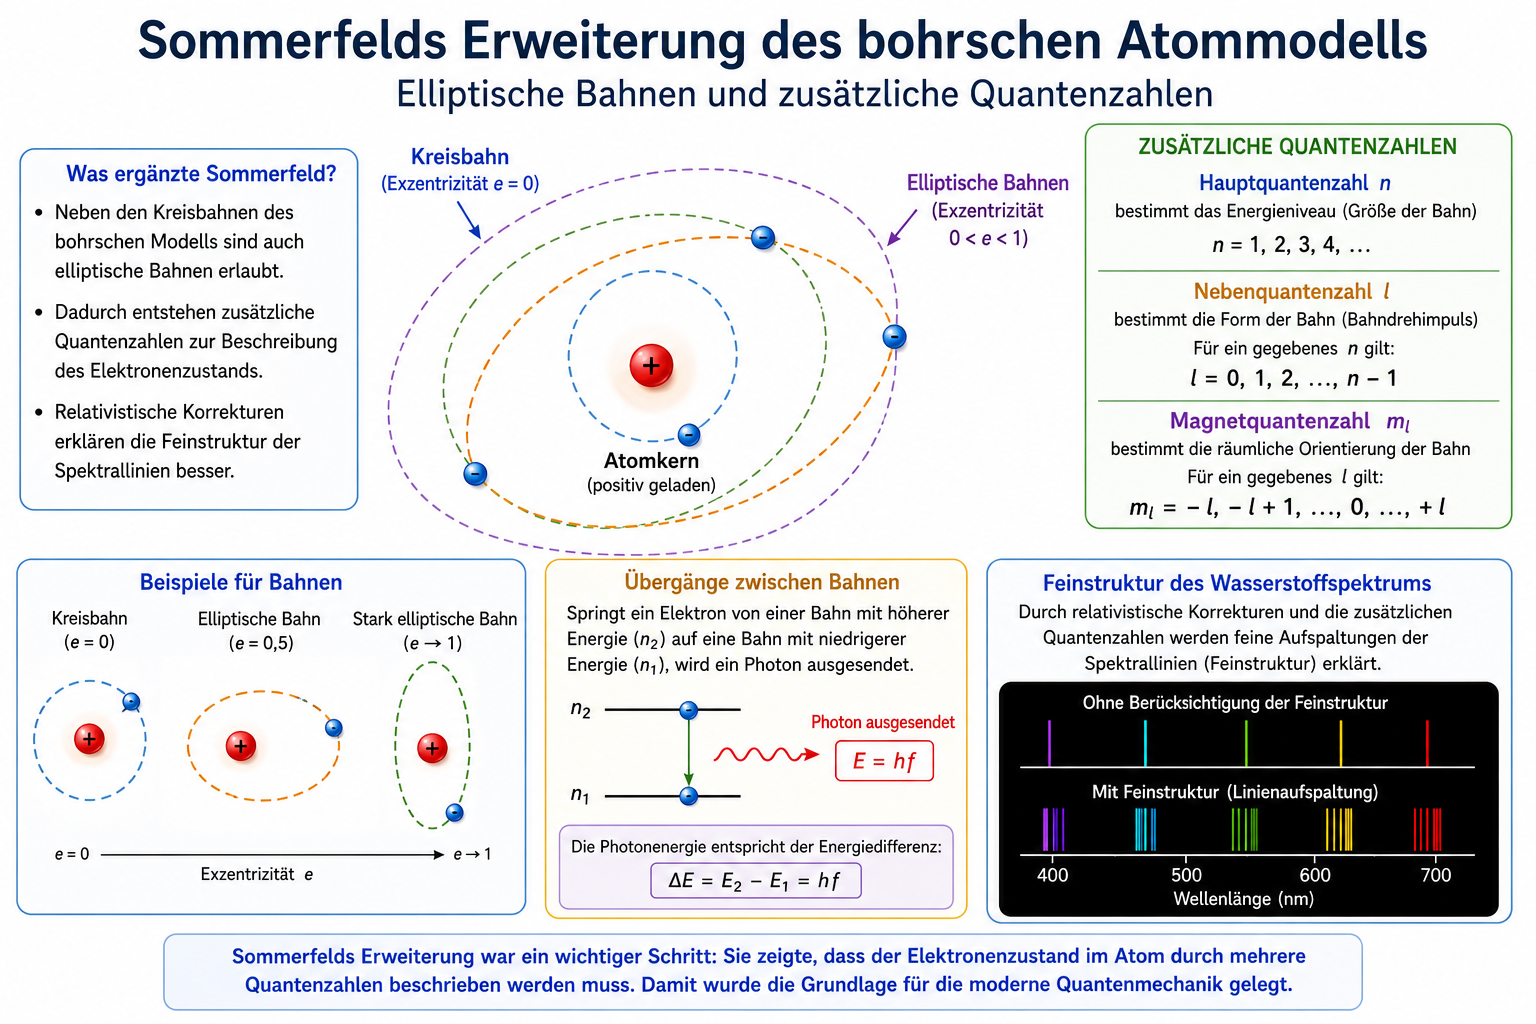
\includegraphics[width=0.75\textwidth]{bilder/elliptische_bahnen}
	\caption{Schematische Darstellung der Sommerfeld-Erweiterung des bohrschen
		Atommodells. Neben Kreisbahnen werden auch elliptische Elektronenbahnen
		zugelassen. Dadurch entstehen zusätzliche Quantenzahlen zur Beschreibung
		der Bahnform.}
	\label{fig:sommerfeld_atommodell}
\end{figure}

Im bohrschen Modell wurde die Bahn des Elektrons im Wesentlichen durch eine
Quantenzahl beschrieben. Diese Hauptquantenzahl \(n\) bestimmte das
Energieniveau. Sommerfeld führte weitere Quantenzahlen ein, um zusätzliche
Eigenschaften der Elektronenbahn zu erfassen. Dazu gehörte insbesondere eine
Quantenzahl für die Form der Bahn.

Die Hauptquantenzahl \(n\) beschreibt weiterhin die Größe beziehungsweise das
Energieniveau der Bahn:

\[
n = 1,2,3,\ldots
\]

Zusätzlich tritt eine weitere Quantenzahl auf, die mit der Form der Bahn
zusammenhängt. In der späteren Quantenmechanik wird diese Idee zur
Nebenquantenzahl beziehungsweise Bahndrehimpulsquantenzahl weiterentwickelt.

Anschaulich kann man sagen: Bei Bohr gab es zu einem bestimmten Energieniveau
eine einfache Kreisbahn. Bei Sommerfeld können zu einem Energieniveau
verschiedene Bahnformen gehören. Das Elektron erhält dadurch zusätzliche
Möglichkeiten, ohne dass das Modell seine Grundidee der Quantisierung aufgibt.

Ein weiterer wichtiger Punkt war die Berücksichtigung relativistischer Effekte.
Bei Elektronenbahnen nahe am Kern können die Geschwindigkeiten des Elektrons so
groß werden, dass kleine Korrekturen aus der speziellen Relativitätstheorie
notwendig werden. Sommerfeld konnte damit bestimmte Feinheiten im
Wasserstoffspektrum besser erklären.

Diese feinen Aufspaltungen nennt man Feinstruktur. Sie zeigen, dass die
Spektrallinien nicht immer einfache einzelne Linien sind, sondern bei genauerer
Messung aus mehreren nahe beieinanderliegenden Linien bestehen können. Das
Sommerfeld-Modell war ein wichtiger Versuch, diese feinere Struktur innerhalb
eines noch anschaulichen Bahnmodells zu verstehen.

Für das Elektron bedeutete Sommerfelds Erweiterung, dass seine Bewegung im Atom
nicht mehr nur durch eine einzige Quantenzahl beschrieben wurde. Das Elektron
erhielt zusätzliche diskrete Eigenschaften. Damit wurde die Vorstellung
vorbereitet, dass der Zustand eines Elektrons im Atom durch mehrere Quantenzahlen
charakterisiert wird.

Trotz dieser Verbesserung blieb auch Sommerfelds Modell ein klassisch
geprägtes Bahnmodell. Es verwendete weiterhin die Vorstellung eines Elektrons,
das sich auf einer bestimmten Bahn um den Kern bewegt. Genau diese Vorstellung
wurde später durch die moderne Quantenmechanik aufgegeben.

Der historische Wert des Sommerfeld-Modells liegt daher in seiner
Übergangsrolle. Es zeigte, dass Bohrs einfache Quantisierung nicht ausreichte
und dass der Elektronenzustand im Atom durch mehrere diskrete Größen beschrieben
werden muss. Damit führte es direkt zur quantenmechanischen Beschreibung der
Elektronenhülle.

\begin{DidacticBox}[Warum Sommerfeld Bohr erweitern musste]
	
	\label{box:sommerfeld-erweiterung}
	Bohrs Modell erklärte das Wasserstoffatom, aber nicht alle feinen Details der
	Spektrallinien. Sommerfeld erweiterte das Modell deshalb durch elliptische
	Bahnen, zusätzliche Quantenzahlen und relativistische Korrekturen.
	
	Damit wurde klar: Der Zustand eines Elektrons im Atom lässt sich nicht mehr
	durch nur eine einzige Quantenzahl beschreiben.
	
\end{DidacticBox}